\documentclass[8pt]{beamer}
\usepackage[T2A]{fontenc}                
\usepackage[utf8]{inputenc}  
\usepackage[english, russian]{babel}
\usepackage{indentfirst}
\usepackage{amsmath}
\usepackage[english, russian]{babel}

\usetheme{Frankfurt}
\usecolortheme{seahorse}

\title{Задание 4}
\author{Блохина Анна \\ Нагаева Варвара \\ Некрасова Мария \\ Смирнов Александр}
\date{Апрель 2018}

\begin{document}
\frame{\titlepage}

\section{Introduction}
\begin{frame}{Описание задания}
Два поставщика стали -- это компании {Westeros Inc.} и {Harpy \& Co}. Каждая из них предлагает ощутимую скидку при заключении эксклюзивного договора на поставку.\\
Требуется принять объективное решение вопроса о том, с какой из компаний следует заключить договор на поставку стали.\\
Имеются записи о производстве мечей каждым из кузнецов-безупречных, а также данные о количестве сломанных мечей в каждый из месяцев ведения боевых действий.\\
\end{frame}

\begin{frame}{Подход к решению}
Для выбора наилучшего поставщика стали был проведен разведовательный анализ данных. Далее будут приведены его результаты.\\
Проведенный анализ заключает в себе визуализацию данных в виде графиков и диаграм, а также поиск критерия для оптимального решения.\\
\center{$J = C_s - C_d - Fine,$}\\
Где $C_s$ и $C_d$ -- это некоторые нормированные константы, доля максимального результата для проданного товара и некачественного соответственно, $Fine$ - штраф.
\end{frame}

\begin{frame}{Количество произведенных мечей}
\begin{figure}[h]
\center{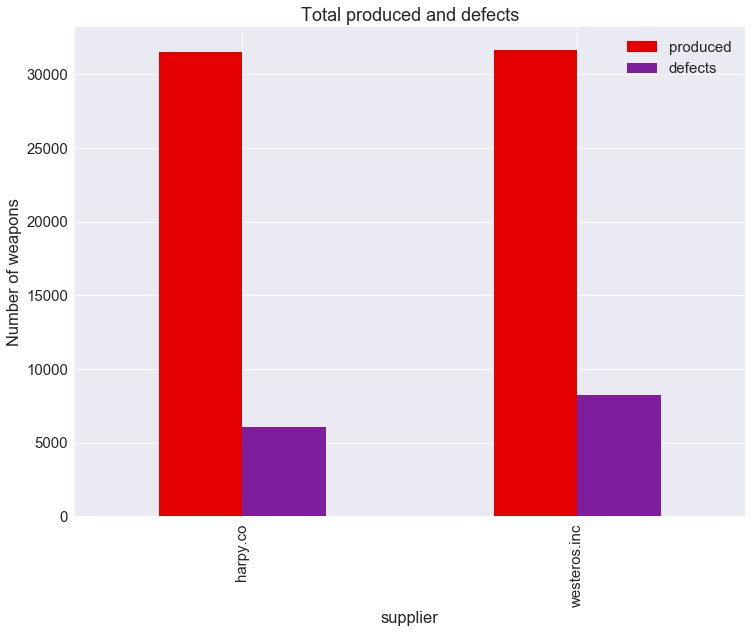
\includegraphics[width=1\linewidth]{img/1.png}}
\label{ris:1.png}
\end{figure}
Компания {Westeros Inc.} производит больше стали чем {Harpy \& Co} в течение первых 5 месяцев. В 6 месяце - наоборот.
\end{frame}

\begin{frame}{Константа $C_s$}
\begin{figure}[h]
\center{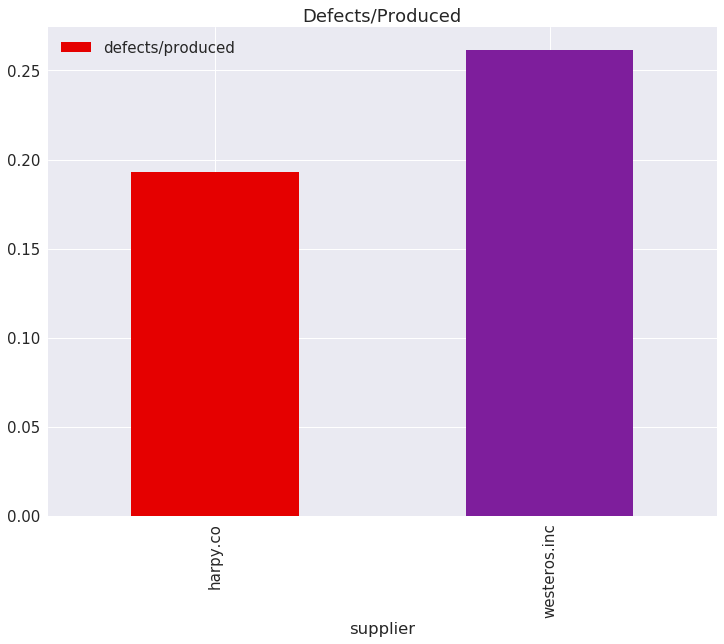
\includegraphics[width=1\linewidth]{img/2.png}}
\label{ris:2.png}
\end{figure}
Построим функцию $P_{max}$ такую, что в каждый месяц она принимает максимальное значение из двух возможных.\\
Для каждой фирмы зададим $C_s = 1 - \overline{(\frac{P_{max} - P}{P_{max}})}$\\
$C_s(H) = 0.9960259$\\
$C_s(W) = 0.9989544$
\end{frame}

\begin{frame}{Количество произведенных мечей}
\begin{figure}[h]
\center{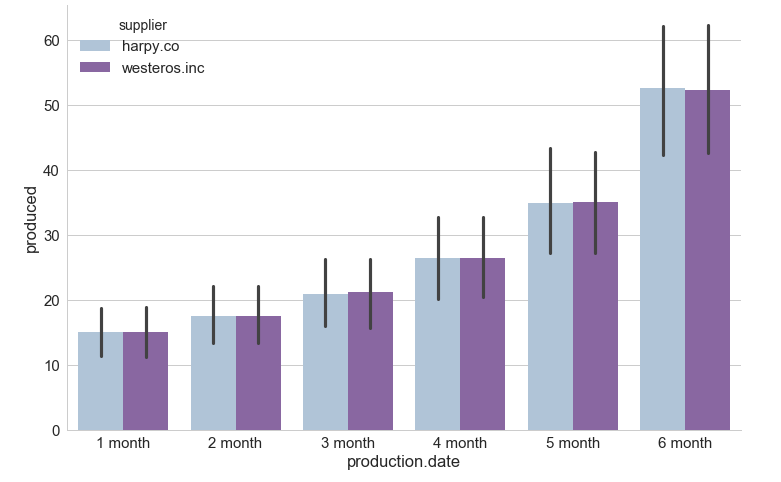
\includegraphics[width=1\linewidth]{img/3.png}}
\label{ris:3.png}
\end{figure}
Наглядная диаграмма произведенного товара. Широкие полосы показывают среднее значение для каждого месяца, узкие - разброс данных.\\
\end{frame}

\begin{frame}{Количество сломанных мечей}
\begin{figure}[h]
\center{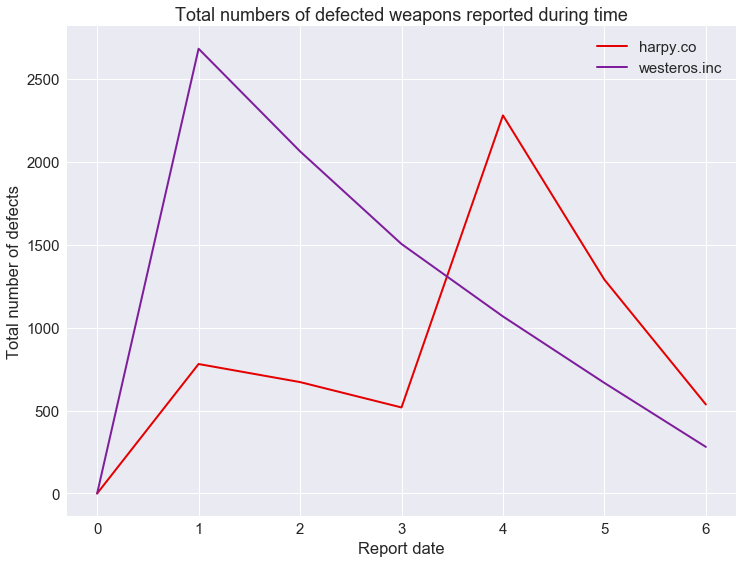
\includegraphics[width=1\linewidth]{img/4.png}}
\label{ris:4.png}
\end{figure}
Видим, что при разности в производстве 30 +- 20, разность в поломке мечей значительно больше:  400 +- 200. \\
Следовательно, за все время у {Westeros Inc.} деталей ломается больше, чем у {Harpy \& Co} при примерно одинаковой производительности.
\end{frame}

\begin{frame}{Константа $C_d$}
\begin{figure}[h]
\center{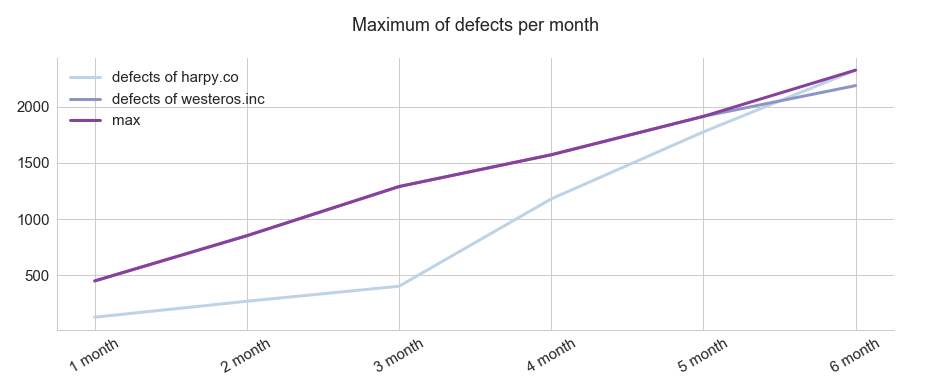
\includegraphics[width=1\linewidth]{img/5.png}}
\label{ris:5.png}
\end{figure}
Построим функцию $D_{max}$ такую, что в каждый месяц она принимает максимальное значение из двух возможных.\\
Для каждой фирмы зададим $C_d = 1 - \overline{(\frac{D_{max} - D}{D_{max}})}$\\
$C_d(H) = 0.5974836$\\
$C_d(W) = 0.9901160$
\end{frame}

\begin{frame}{Среднее число сломанных мечей в месяц}
\begin{figure}[h]
\center{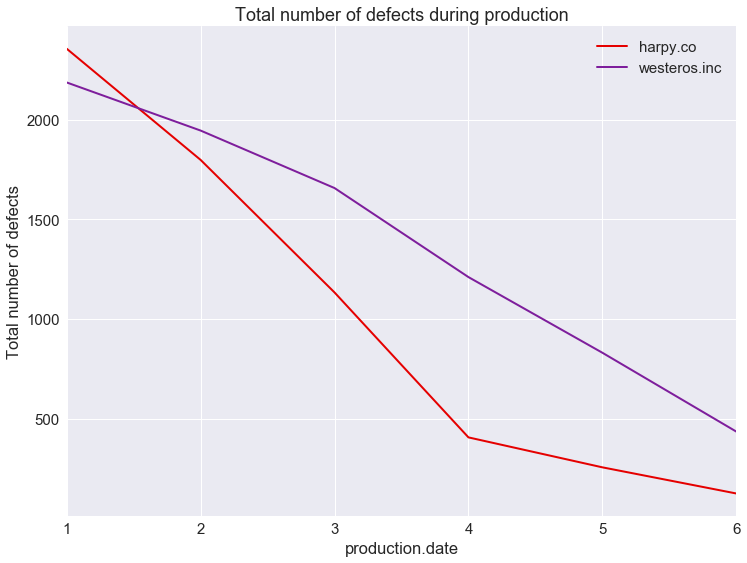
\includegraphics[width=1\linewidth]{img/6.png}}
\label{ris:6.png}
\end{figure}
Компания {Harpy \& Co} в последние месяцы сделала упор на количество, а не качество. Усредненные результаты критерия не покажут такого выброса, но мы учтем этот показатель как штраф, $Fine(H) = J(H) * 0.1$
\end{frame}

\begin{frame}{Среднее число сломанных мечей в месяц}
\begin{figure}[h]
\center{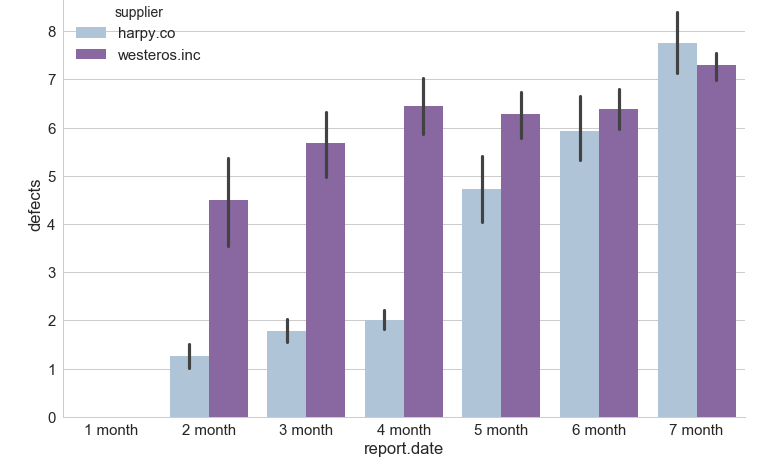
\includegraphics[width=1\linewidth]{img/7.png}}
\label{ris:7.png}
\end{figure}
\end{frame}

\begin{frame}{Отношение количества бракованных деталей к произведенным}
\begin{figure}[h]
\center{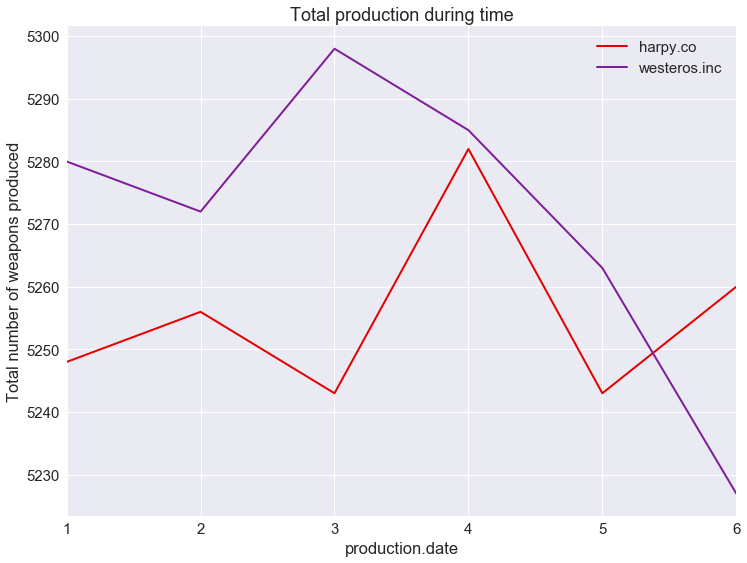
\includegraphics[width=1\linewidth]{img/8.png}}
\label{ris:8.png}
\end{figure}
\end{frame}

\begin{frame}{Вывод}
Подсчитав критерий J для каждой из компаний, получаем, что эксклюзивный договор выгоднее заключить с "Harpy \& Co":\\
\begin{figure}[h]
\begin{minipage}[h]{0.49\linewidth}
\center{
\includegraphics[width=0.5\linewidth]{img/H.jpg} \\ Meereen \\ $J(H) = 0.358688$}
\end{minipage}
\hfill
\begin{minipage}[h]{0.49\linewidth}
\center{
\includegraphics[width=0.5\linewidth]{img/W.jpg} \\ King's Landing \\ $J(W) = 0.008838$}
\end{minipage}
\label{ris:image9}
\end{figure}
\end{frame}


\end{document}

